\section{Operações Binárias}

\begin{frame}[fragile]{Operações bit a bit}

    \begin{itemize}
        \item As operações \textit{bit} a \textit{bit} se comportam da mesma maneira do que
            suas equivalentes da lógica booleana, considerando o valor 0 (zero) como falso e
            1 (um) como verdadeiro

        \item As representações binárias dos operandos devem estar alinhadas (com o mesmo número
            de dígitos) antes da operação (zeros à esquerda podem ser necessários)

        \item A operação \code{c}{&} (e, \textit{and}) resulta em verdadeiro somente quando
            os dois valores são verdadeiros 

        \item A operação \code{c}{|} (ou, \textit{or}) resulta em falso somente quando
            os dois valores são falsos

        \item A operação $\land$ (ou exclusivo, \textit{xor}) resulta em falso somente quando
            ambos valores são iguais

        \item A operação $\sim$ (negação, \textit{not}) é unária, e inverte todos os
            \textit{bits} do operando
    \end{itemize}

\end{frame}

\begin{frame}[fragile]{Visualização das operações bit a bit}

    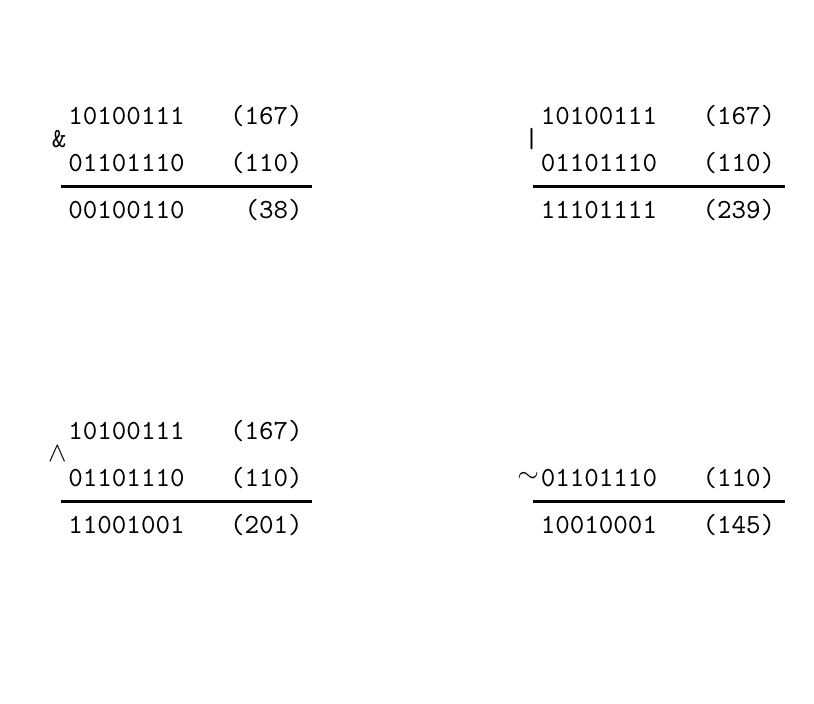
\begin{tikzpicture}
        
        \node[opacity=0] at (0, 4) { };

        \begin{scope}
            \node[opacity=0] at (0, 0) { };

            \node[anchor=east] at (2, 3) {  \texttt{10100111} };
            \node[anchor=east] at (3.5, 3) {  \texttt{(167)} };
            \node[anchor=east] at (2, 2.4) {  \texttt{01101110} };
            \node[anchor=east] at (3.5, 2.4) {  \texttt{(110)} };
            \node[anchor=east] at (0.5, 2.7) {  \texttt{\&} };

            \draw[thick] (0.3, 2.1) -- (3.5, 2.1);

            \node[anchor=east] at (2, 1.8) {  \texttt{00100110} };
            \node[anchor=east] at (3.5, 1.8) {  \texttt{(38)} };
        \end{scope}

        \begin{scope}[shift={(6,0)}]
            \node[opacity=0] at (0, 0) { };

            \node[anchor=east] at (2, 3) {  \texttt{10100111} };
            \node[anchor=east] at (3.5, 3) {  \texttt{(167)} };
            \node[anchor=east] at (2, 2.4) {  \texttt{01101110} };
            \node[anchor=east] at (3.5, 2.4) {  \texttt{(110)} };
            \node[anchor=east] at (0.5, 2.7) {  \texttt{|} };

            \draw[thick] (0.3, 2.1) -- (3.5, 2.1);

            \node[anchor=east] at (2, 1.8) {  \texttt{11101111} };
            \node[anchor=east] at (3.5, 1.8) {  \texttt{(239)} };
        \end{scope}

        \begin{scope}[shift={(0,-4)}]
            \node[opacity=0] at (0, 0) { };

            \node[anchor=east] at (2, 3) {  \texttt{10100111} };
            \node[anchor=east] at (3.5, 3) {  \texttt{(167)} };
            \node[anchor=east] at (2, 2.4) {  \texttt{01101110} };
            \node[anchor=east] at (3.5, 2.4) {  \texttt{(110)} };
            \node[anchor=east] at (0.5, 2.7) {  $\land$ };

            \draw[thick] (0.3, 2.1) -- (3.5, 2.1);

            \node[anchor=east] at (2, 1.8) {  \texttt{11001001} };
            \node[anchor=east] at (3.5, 1.8) {  \texttt{(201)} };
        \end{scope}

        \begin{scope}[shift={(6,-4)}]
            \node[opacity=0] at (0, 0) { };

%            \node[anchor=east] at (2, 3) {  \texttt{10100111} };
%            \node[anchor=east] at (3.5, 3) {  \texttt{(167)} };
            \node[anchor=east] at (2, 2.4) {  \texttt{01101110} };
            \node[anchor=east] at (3.5, 2.4) {  \texttt{(110)} };
            \node[anchor=east] at (0.5, 2.4) {  $\sim$ };

            \draw[thick] (0.3, 2.1) -- (3.5, 2.1);

            \node[anchor=east] at (2, 1.8) {  \texttt{10010001} };
            \node[anchor=east] at (3.5, 1.8) {  \texttt{(145)} };
        \end{scope}



    \end{tikzpicture}

\end{frame}

\begin{frame}[fragile]{Deslocamentos binários}

    \begin{itemize}
        \item O operator \code{c}{<<} (deslocamento à esquerda, \textit{left shift}) adiciona
            o número indicado ($k$) de zeros à esquerda do número

        \item A operação equivale à uma multiplicação por $2^k$, levando em conta um possível
            \textit{overflow} 

        \item O operator \code{c}{>>} (deslocamento à direita, \textit{right shift}) adiciona
            o número indicado ($k$) de zeros à direita do número

        \item A mesma quantidade de \textit{bits} à direita são desprezados

        \item Se o sinal é propagado, a operação é denominada deslocamento à direita aritmético;
            caso contrário, deslocamenteo à direita binário

        \item No caso do operador aritmético, a operação equivale à uma divisão inteira 
            euclidiana por $2^k$

        \item Em C/C++, o operador \code{c}{>>} é aritmético, e a divisão inteira (\code{c}{/})
            não é euclidiana (é a divisão de menor resto)
    \end{itemize}

\end{frame}

\begin{frame}[fragile]{Exemplo de deslocamentos binários}
    \inputcode{c++}{shift.cpp}
\end{frame}

\begin{frame}[fragile]{Máscaras binárias}

    \begin{itemize}
        \item Uma máscara binária é um padrão binário que permite a localização, extração ou
            alteração de determinados \textit{bits} de uma representação binária

        \item A máscara \code{c}{(1 << k)} corresponde a todos os \textit{bits} iguais a zero,
            exceto o $k$-ésimo \textit{bit}, que é igual a um

        \item Esta máscara permite a leitura do $k$-ésimo \textit{bit} de um número através do
            operador \code{c}{&}

        \item Esta mesma máscara permite ligar o $k$-ésimo \textit{bit} de um número através do 
            operador \code{c}{|}

        \item A negação desta máscara ($\sim$\code{c}{(1 << k)}) permite desligar o $k$-ésimo
            \textit{bit} de um número com o operador \code{c}{&}

        \item A máscara \code{c}{((1 << k) - 1)} permite a extração dos $k$ \textit{bits} menos
            significativos de um número através do operador \code{c}{&}
    \end{itemize}

\end{frame}

\begin{frame}[fragile]{Exemplo de uso de máscaras binárias}
    \inputcode{c++}{rotate.cpp}
\end{frame}

\begin{frame}[fragile]{Bit menos significativo}

    \begin{itemize}
        \item O \textit{bit} menos significativo (\textit{least significant bit -- LSB}) de um 
            inteiro $n$ pode ser extraído em $O(1)$

        \item Basta fazer a conjunção de $n$ com seu simétrico $-n$

        \item Em termos de código, \code{c}{LSB(n) = n & -n}

        \item É possível desligar o LSB com a expressão \code{c}{(n &} $\sim$\code{c}{(1 << LSB(n))}

        \item Porém a expressão \code{c}{CLSB(n) = n & (n - 1)} gera o mesmo resultado usando uma
            sintaxe mais simples e eficiente

        \item A rotina \code{c}{CLSB(n)} pode ser usada para contar o número de \textit{bits} 
            ligados de $n$ em $O(\log n)$

    \end{itemize}

\end{frame}

\begin{frame}[fragile]{Exemplo de rotinas com LSB em C++}
    \inputsnippet{c}{1}{20}{lsb.cpp}
\end{frame}

\begin{frame}[fragile]{Exemplo de rotinas com LSB em C++}
    \inputsnippet{c}{21}{41}{lsb.cpp}
\end{frame}

\begin{frame}[fragile]{Funções do GCC}

    \begin{itemize}
        \item O GCC oferece uma série de funções de baixo nível para manipulação
            binária

        \item A função \code{c}{__builtin_popcount(x)} retorna o número de \textit{bits} ligados
            de $x$

        \item A função \code{c}{__builtin_clz(x)} o número de zeros à esquerda na representação
            binária de $x$ (\textit{clz -- count leading zeroes})

        \item A função \code{c}{__builtin_ctz(x)} o número de zeros à direita na representação
            binária de $x$ (\textit{ctz -- count trailing zeroes})

        \item As duas funções anteriores tem comportamento indefinido se $x$ é igual a zero

        \item A função \code{c}{__builtin_ffs(x)} retorna 1 mais o índice do \textit{bit} 
            menos significativo de $x$, ou zero, se $x$ é igual a zero

    \end{itemize}

\end{frame}

\begin{frame}[fragile]{Exemplo de uso das funções do GCC}
    \inputcode{c++}{gcc.cpp}
\end{frame}
